% Progress report for the supervisor: gamma-CsPbI3 iodine vacancies
% Build: pdflatex presentation.tex (run twice). Figures are read from ../assets/.
\documentclass[aspectratio=169,10pt]{beamer}
\usetheme[progressbar=frametitle,numbering=fraction]{metropolis}
\usepackage[utf8]{inputenc}
\usepackage[T1]{fontenc}
\usepackage{booktabs}
\usepackage{graphicx}
\usepackage{xcolor}
\graphicspath{{../assets/}}

\definecolor{pb}{HTML}{7F77DD}
\definecolor{iod}{HTML}{D85A30}
\definecolor{cs}{HTML}{1D9E75}
\setbeamercolor{alerted text}{fg=iod}
\newcommand{\cpi}{$\gamma$-CsPbI$_3$}
\newcommand{\done}{\textcolor{cs}{\textbf{done}}}
\newcommand{\run}{\textcolor{iod}{\textbf{running}}}
\newcommand{\nxt}{\textcolor{gray}{next}}
\renewcommand{\arraystretch}{1.15}

% ---------- references: [n] marks in text, full entries at the foot of each slide ----------
\newcommand{\cit}[1]{\textsuperscript{\textcolor{gray}{[#1]}}}
\newcommand{\refs}[1]{\par\vfill\begingroup\tiny\color{gray}\raggedright #1\par\endgroup}
\newcommand{\RA}{[1] A.\,N.~Arber, Vikram, F.\,C.~Mocanu, M.\,S.~Islam, Chem.\ Mater.\ \textbf{37}, 4416 (2025).}
\newcommand{\RB}{[2] R.-I.~Biega, L.~Leppert, J.\ Phys.: Energy \textbf{3}, 034017 (2021).}
\newcommand{\RC}{[3] B.~Ahmad, M.\,S.\,R.~Limon, Z.~Ahmad, Phys.\ Rev.\ Mater.\ \textbf{8}, 125402 (2024).}
\newcommand{\RD}{[4] R.\,J.~Sutton \emph{et al.}, ACS Energy Lett.\ \textbf{3}, 1787 (2018).}
\newcommand{\RE}{[5] J.~Kaczkowski, I.~P{\l}owa\'s-Korus, J.\ Phys.\ Chem.\ Lett.\ \textbf{12}, 6613 (2021).}
\newcommand{\RF}{[6] A.~Seidu \emph{et al.}, J.\ Chem.\ Phys.\ \textbf{154}, 074712 (2021).}
\newcommand{\RG}{[7] N.~Xu \emph{et al.}, Point defects in metal halide perovskites, Nat.\ Rev.\ Mater.\ (2025).}
\newcommand{\RH}{[8] Z.~Wylie \emph{et al.}, ACS Energy Lett.\ \textbf{9}, 4378 (2024).}
\newcommand{\RI}{[9] J.\,P.~Perdew \emph{et al.}, Phys.\ Rev.\ Lett.\ \textbf{100}, 136406 (2008).}
\newcommand{\RJ}{[10] P.~Giannozzi \emph{et al.}, J.\ Phys.: Condens.\ Matter \textbf{21}, 395502 (2009); \textbf{29}, 465901 (2017).}
\newcommand{\RK}{[11] G.~Prandini \emph{et al.}, npj Comput.\ Mater.\ \textbf{4}, 72 (2018).}
\newcommand{\RL}{[12] J.~Even \emph{et al.}, J.\ Phys.\ Chem.\ Lett.\ \textbf{4}, 2999 (2013).}
\newcommand{\RM}{[13] C.~Freysoldt \emph{et al.}, Rev.\ Mod.\ Phys.\ \textbf{86}, 253 (2014).}
\newcommand{\RN}{[14] A.\,J.~Cohen, P.~Mori-S\'anchez, W.~Yang, Science \textbf{321}, 792 (2008).}
\newcommand{\RO}{[15] G.~Henkelman, B.\,P.~Uberuaga, H.~J\'onsson, J.\ Chem.\ Phys.\ \textbf{113}, 9901 (2000).}
\newcommand{\RP}{[16] S.~Smidstrup \emph{et al.}, J.\ Chem.\ Phys.\ \textbf{140}, 214106 (2014).}
\newcommand{\RQ}{[17] A.~Togo, K.~Shinohara, I.~Tanaka, Sci.\ Technol.\ Adv.\ Mater.: Methods \textbf{4}, 2384822 (2024).}
\newcommand{\RR}{[18] A.\,H.~Larsen \emph{et al.}, J.\ Phys.: Condens.\ Matter \textbf{29}, 273002 (2017).}
\newcommand{\RT}{[20] J.~Zhang \emph{et al.}, Appl.\ Surf.\ Sci.\ \textbf{679}, 161235 (2025).}
\newcommand{\RS}{[19] Y.~Huang, W.-J.~Yin, Y.~He, J.\ Phys.\ Chem.\ C \textbf{122}, 1345 (2018).}

\title{Iodine Vacancy Sites and Migration Paths in Bulk \cpi}
\subtitle{Progress report}
\author{Duy M. Dao}
\institute{School of Materials Science and Engineering, Tsinghua University}
\setbeamertemplate{title separator}{\vspace{-0.5em}}
\date{October 2026}

\begin{document}

\maketitle

\begin{frame}{Outline}
  \begin{enumerate}
    \item Motivation
    \item Literature and gap
    \item Methods and why
    \item Results so far
    \item Next steps
  \end{enumerate}
\end{frame}

% =====================================================================
\section{Motivation}

\begin{frame}{Why iodine vacancies?}
  \begin{columns}[T]
    \column{0.55\textwidth}
    \textbf{Halide perovskites: electronically tolerant, ionically weak}
    \begin{itemize}
      \item Most native defects leave no deep traps\cit{7}
      \item But iodine vacancies form easily and \alert{move at room temperature}\cit{1,7}
    \end{itemize}
    \textbf{Moving vacancies cause}
    \begin{itemize}
      \item $J$--$V$ hysteresis and drifting response\cit{7}
      \item Ion pile-up and reactions at contacts
      \item Loss of stability: \cpi\ $\rightarrow$ yellow $\delta$ phase, starting at surface iodide defects\cit{8}
    \end{itemize}
    \column{0.42\textwidth}
    \begin{block}{Goal of the project}
      Migration barriers of the iodine vacancy in \cpi:
      \begin{enumerate}
        \item every distinct hop in the bulk \alert{(this talk)}
        \item layer by layer below the CsI-terminated (001) surface \textcolor{gray}{(later)}
      \end{enumerate}
    \end{block}
  \end{columns}
  \refs{\RA\quad \RG\quad \RH}
\end{frame}

\begin{frame}{\cpi: tilted octahedra make two iodine sites}
  \centering
  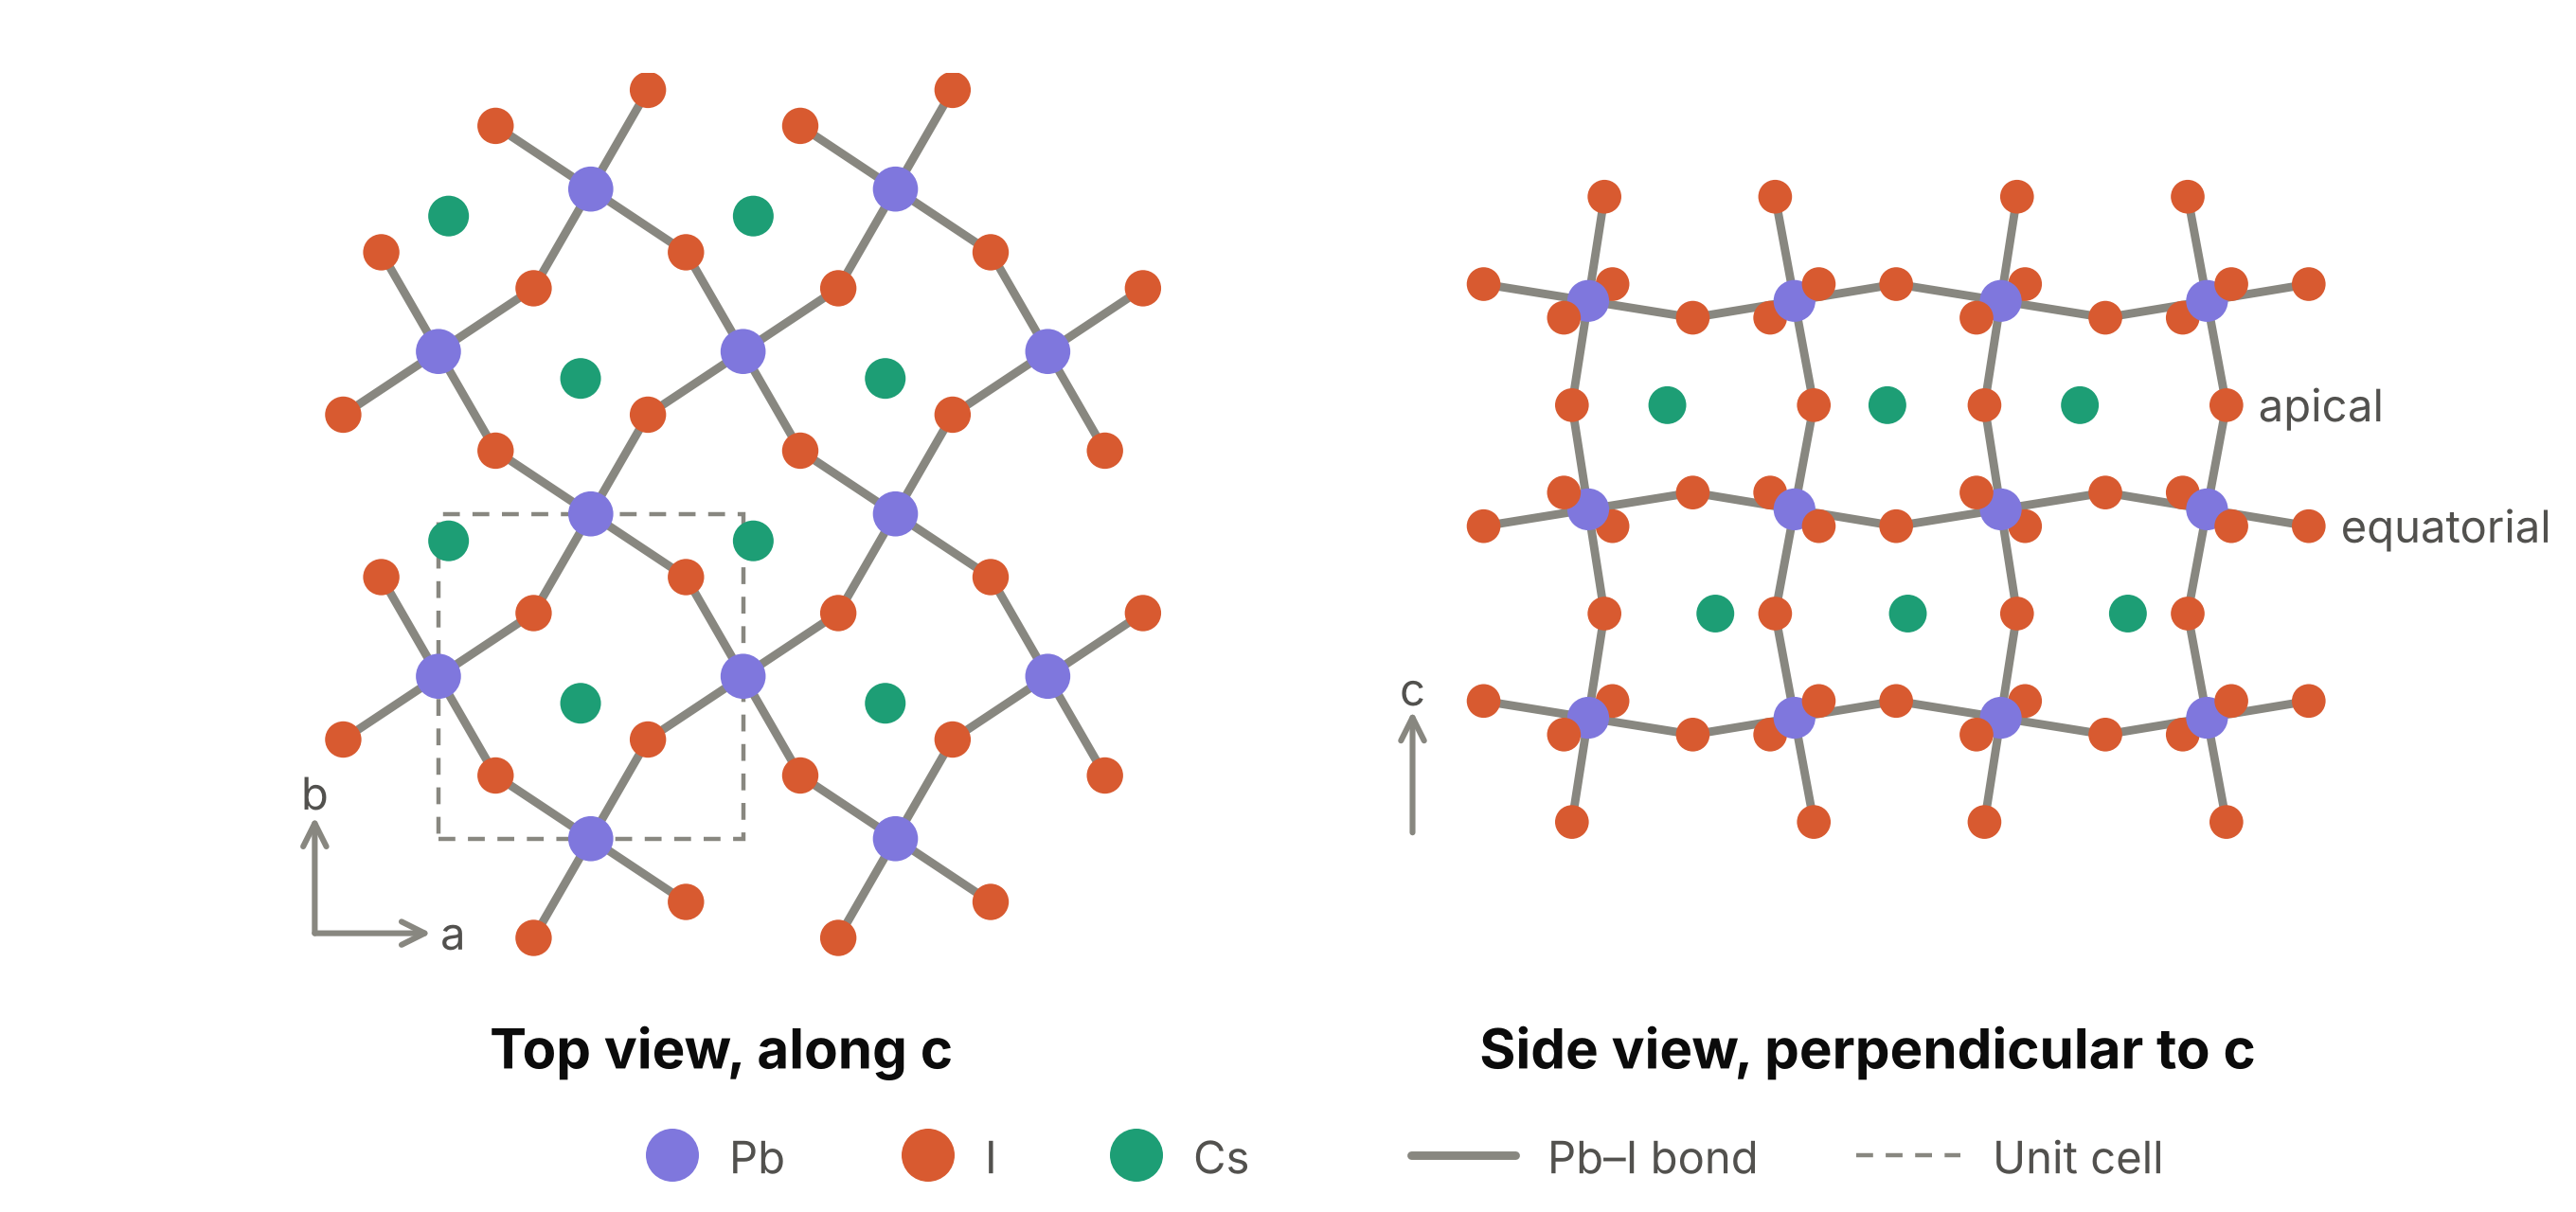
\includegraphics[width=0.45\textwidth]{gamma_CsPbI3_lattice_tilted_octahedra.png}\hfill
  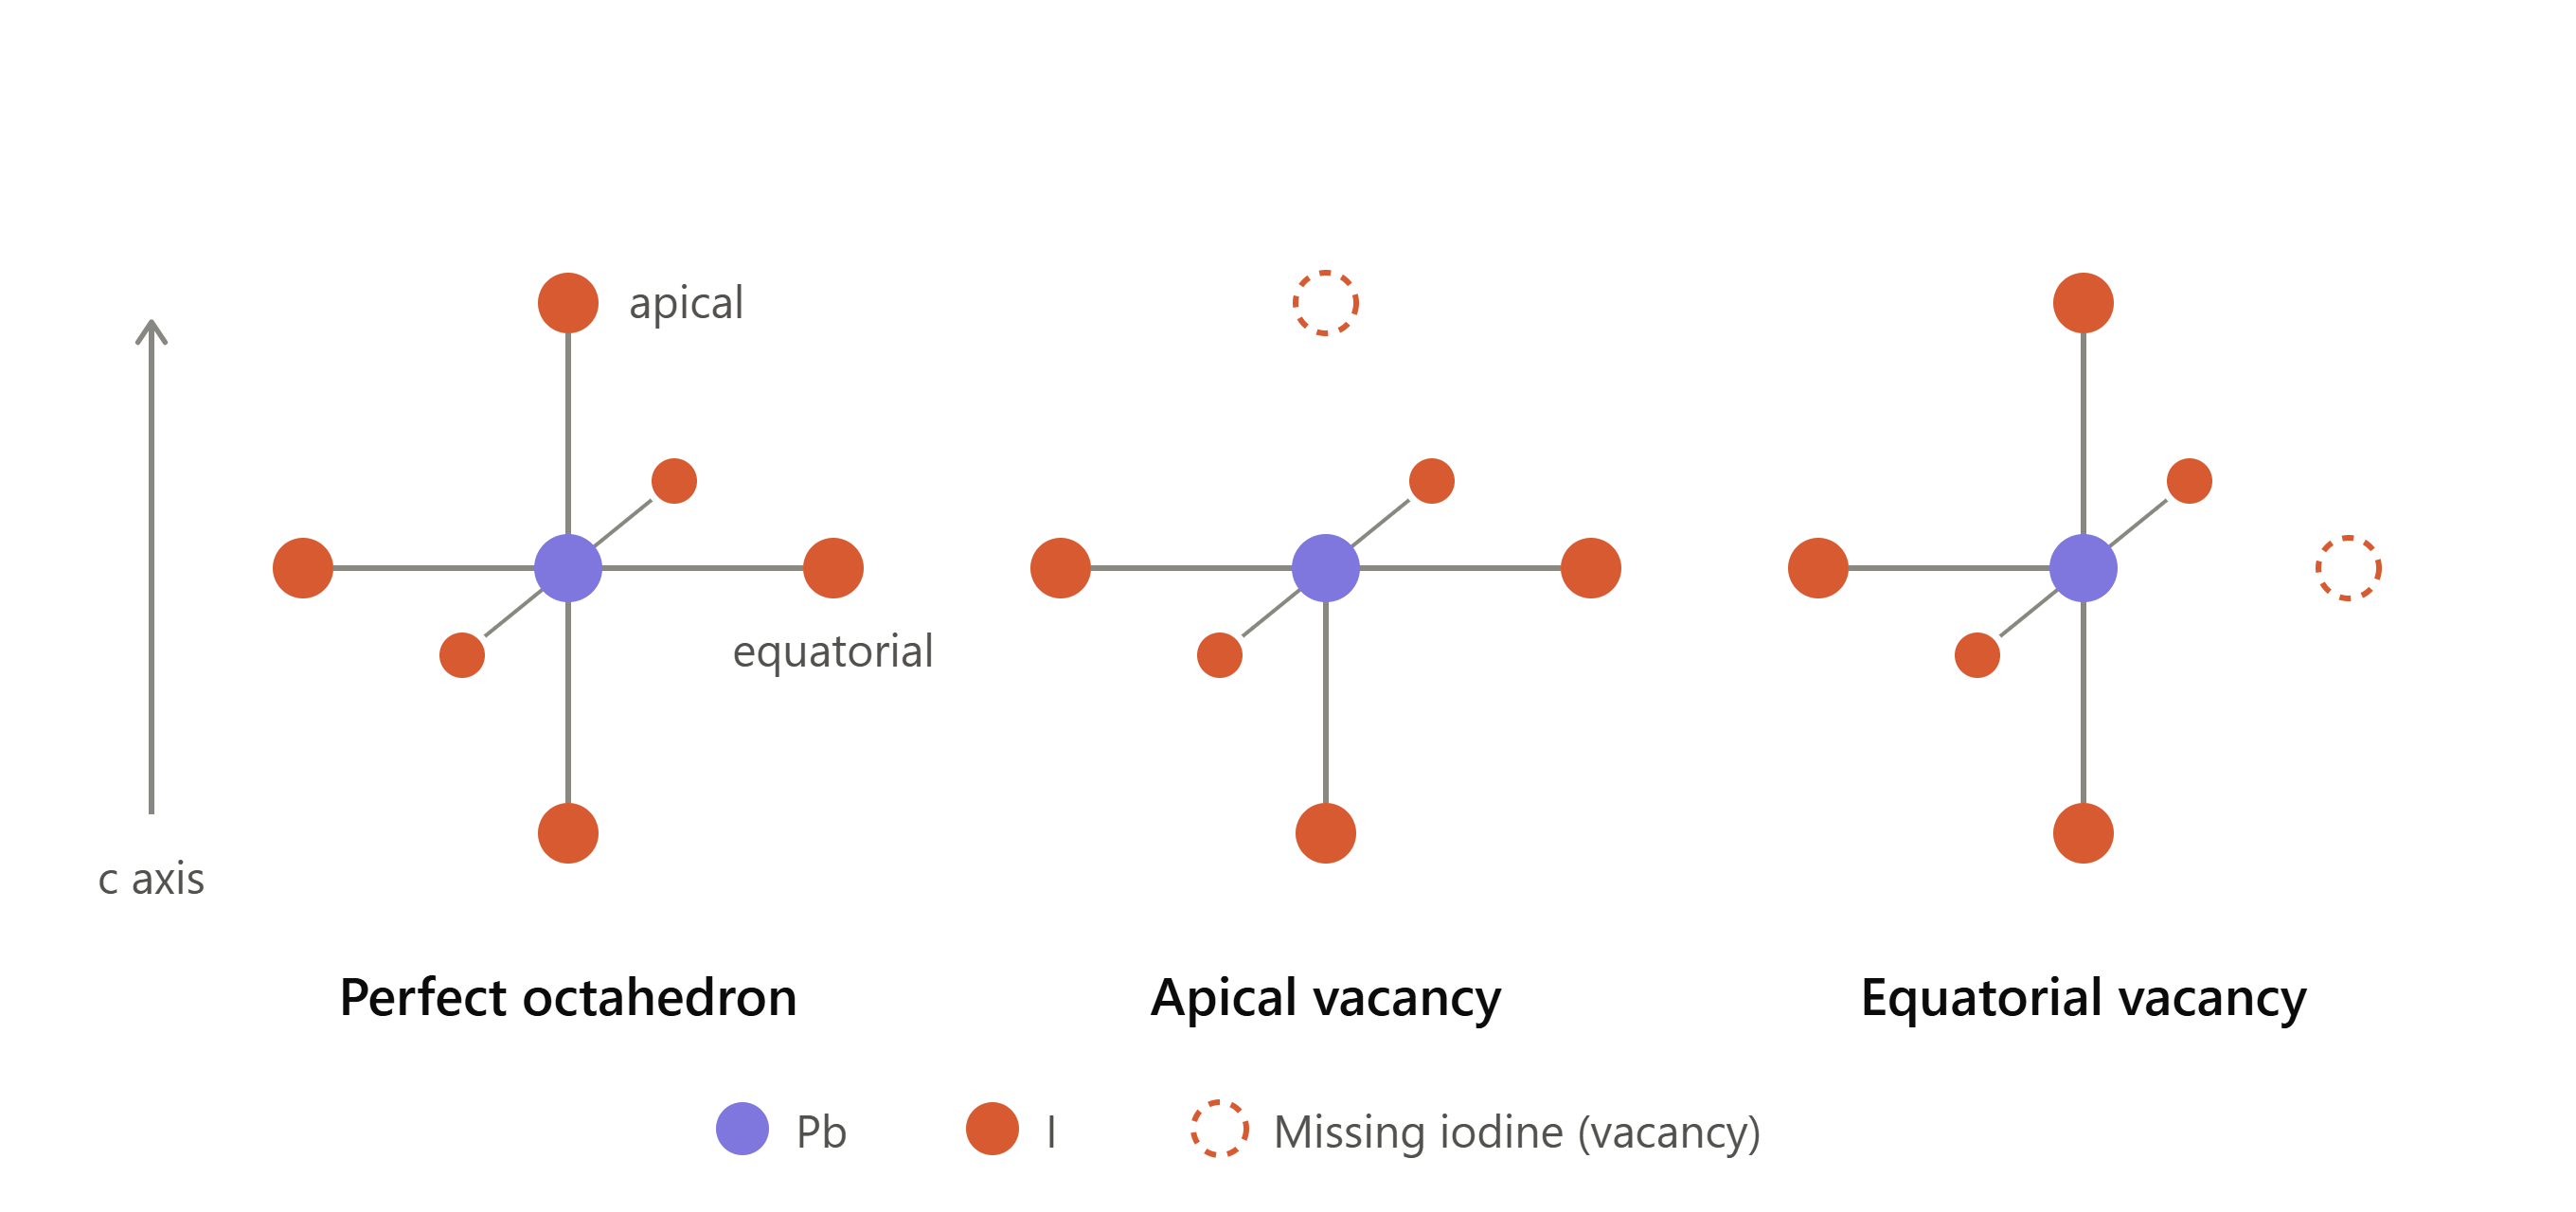
\includegraphics[width=0.45\textwidth]{iodine_vacancy_sites_apical_vs_equatorial.png}

  \vspace{0.3em}
  \small
  \begin{tabular}{ll}
    \toprule
    Space group & Pnma (No.\ 62), 20 atoms per cell\cit{4} \\
    Apical I, \textbf{4c} & links octahedra along $c$, in the CsI layers; Pb--I--Pb $155^\circ$ \\
    Equatorial I, \textbf{8d} & links octahedra in the $ab$ plane, in the PbI$_2$ layers; Pb--I--Pb $148^\circ$ \\
    \bottomrule
  \end{tabular}

  \vspace{0.4em}
  The two sites differ \alert{only through the octahedral tilt} (in the cubic phase they are equivalent).
  \refs{\RD\quad Angles and figures: this work (tight PBEsol relaxation).}
\end{frame}

% =====================================================================
\section{Literature and gap}

\begin{frame}{Key papers}
  \scriptsize
  \begin{tabular}{p{0.19\textwidth}p{0.37\textwidth}p{0.34\textwidth}}
    \toprule
    Paper & What it did & What it leaves open \\
    \midrule
    \textbf{A} Arber 2025\cit{1} \newline \footnotesize Chem.\ Mater. (anchor) & Bulk \cpi, PBEsol, 2$\times$2$\times$2 cell. Barriers 0.34 eV (8d--8d), 0.35 eV (8d--4c), 0.77 eV (4c--4c) & One barrier per path \emph{type}; charge state not stated; no surface \\
    \addlinespace
    \textbf{B} Biega 2021\cit{2} \newline \footnotesize J.\ Phys.\ Energy & Cubic CsPbBr$_3$ slabs: long axial jump about half the bulk barrier at the surface & Long jump only; no tilt; thin, partly frozen slab never returns to bulk \\
    \addlinespace
    \textbf{C} Ahmad 2024\cit{3} \newline \footnotesize Phys.\ Rev.\ Mater. & CsPbI$_3$, 17-layer slab: vacancy formation energies vs depth & No barriers; equatorial sites only; slab interior off from own bulk by 0.05--0.66 eV \\
    \addlinespace
    \textbf{D} Zhang 2025\cit{20} \newline \footnotesize Appl.\ Surf.\ Sci. & Bulk \cpi\ under strain, PBEsol: two paths, 0.51 eV (edge, towards apical) and 0.54 eV (in-plane); rectangular cell (PBEsol, PBE, HSE06) & Charge state; site energies; only two paths \\
    \bottomrule
  \end{tabular}

  \vspace{0.2em}
  \footnotesize\textbf{Gap:} no iodine-vacancy barriers in \cpi\ resolved by hop and by depth, in a slab whose interior reproduces the bulk.
  \refs{\RA\quad \RB\quad \RC\quad \RT}
\end{frame}

\begin{frame}{Gaps and research questions}
  \footnotesize
  \begin{tabular}{lp{0.42\textwidth}p{0.38\textwidth}}
    \toprule
    & Gap & Research question \\
    \midrule
    \textbf{G1} & Bulk barriers known per path type only; charge state unstated\cit{1} & \textbf{RQ1} Which site does the vacancy prefer, in each charge state? \newline \textbf{RQ2} Bulk barriers, and how the number and direction of hops shape transport (ab plane vs $c$)? \\
    \addlinespace
    \textbf{G2} & Surface effect known for one jump in cubic CsPbBr$_3$ only\cit{2} & \textbf{RQ3--4} Barriers and drift direction layer by layer below the surface \\
    \addlinespace
    \textbf{G3} & Neither surface study recovers its own bulk\cit{2,3} & \textbf{RQ5} Does the slab middle reproduce the bulk? \\
    \bottomrule
  \end{tabular}

  \vspace{0.2em}
  \textbf{Scope:} iodine vacancy only; charge $+1$ and neutral; CsI termination. \\
  Interstitials, PbI$_2$ termination, formation energies vs $\mu_\mathrm{I}$ and $E_F$, ML potentials: \emph{out of scope for now}.

  \vspace{0.2em}
  \alert{This talk: G1 (RQ1 done for $+1$, nearly done for neutral; RQ2 set up).}
  \refs{\RA\quad \RB\quad \RC}
\end{frame}

% =====================================================================
\section{Methods and why}

\begin{frame}{Workflow}
  \footnotesize
  \begin{tabular}{clll}
    \toprule
    Step & Calculation & Purpose & Status \\
    \midrule
    1 & Unit cell: convergence, tight relaxation & Reference lattice & \done \\
    2 & Perfect 2$\times$2$\times$2 supercell (160 atoms) & Energy reference & \done \\
    3 & 4c and 8d vacancy, $+1$ and 0 & Site preference (RQ1) & 3/4 \done, 1 \run \\
    4 & NEB, 10 distinct bulk hops & Bulk barriers (RQ2) & inputs ready, \nxt \\
    5 & CsI-terminated (001) slab & Bulk-like slab middle & \nxt \\
    6 & Vacancies at increasing depth & Site energy vs depth & \nxt \\
    7 & NEB at increasing depth & Barriers vs depth & \nxt \\
    \bottomrule
  \end{tabular}

  \vspace{0.8em}
  Steps 1--4 are the bulk reference that every slab result is compared against.
\end{frame}

\begin{frame}{Settings and why}
  \footnotesize
  \begin{tabular}{lll}
    \toprule
    Choice & Value & Why \\
    \midrule
    Code & Quantum ESPRESSO 6.5\cit{10} & One version for all production runs \\
    Functional & PBEsol\cit{9} & Good solid-state lattices; \textbf{same as paper A}\cit{1} \\
    Spin--orbit & Not included & Mainly shifts the Pb-$p$ band\cit{12}; check later \\
    Dispersion & None & Same as paper A\cit{1} \\
    Pseudopotentials & SSSP 1.3 PBEsol efficiency\cit{11} & Verified library \\
    Cutoff & 60 Ry (480 Ry density) & 0.86 meV/atom from 80 Ry \\
    $k$-mesh & 4$\times$4$\times$3 cell; 2$\times$2$\times$2 supercell & 0.23 meV/atom from 6$\times$6$\times$4; same density \\
    Forces & largest $< 0.01$ eV/\AA & Same as paper A\cit{1} \\
    \bottomrule
  \end{tabular}

  \vspace{0.6em}
  Guiding rule: \alert{match paper A where possible}, so any difference in results is physics, not settings.
  \refs{\RA\quad \RI\quad \RJ\quad \RK\quad \RL\quad Cutoff and $k$-mesh: this work (next slide).}
\end{frame}

\begin{frame}{Convergence tests (20-atom cell)}
  \begin{columns}[T]
    \column{0.45\textwidth}
    \centering\small
    \begin{tabular}{lc}
      \toprule
      $k$-mesh (50 Ry) & meV/atom vs 6$\times$6$\times$4 \\
      \midrule
      2$\times$2$\times$1 & 45.46 \\
      3$\times$3$\times$2 & 2.52 \\
      \textbf{4$\times$4$\times$3} & \textbf{0.23} \\
      5$\times$5$\times$4 & 0.004 \\
      \bottomrule
    \end{tabular}
    \column{0.5\textwidth}
    \centering\small
    \begin{tabular}{lcc}
      \toprule
      Cutoff & meV/atom vs 80 Ry & $P$ (kbar) \\
      \midrule
      40 Ry & 5.83 & $-1.89$ \\
      50 Ry & 3.29 & $-1.57$ \\
      \textbf{60 Ry} & \textbf{0.86} & $\mathbf{-1.48}$ \\
      70 Ry & 0.40 & $-1.35$ \\
      80 Ry & 0 & $-1.39$ \\
      \bottomrule
    \end{tabular}
  \end{columns}

  \vspace{1em}
  Both choices are well below 1 meV/atom, far smaller than the energy differences we compare (tens of meV and more).
  \refs{All values: this work (Quantum ESPRESSO 7.6, PBEsol, SSSP).}
\end{frame}

\begin{frame}{Unit-cell relaxation}
  \centering\small
  \begin{tabular}{lcccc}
    \toprule
    & $a$ (\AA) & $b$ (\AA) & $c$ (\AA) & Volume (\AA$^3$) \\
    \midrule
    Experiment, 293 K\cit{4} & 8.577 & 8.856 & 12.472 & 947.3 \\
    Soft relaxation & 8.378 & 8.933 & 12.352 & 924.4 \\
    \textbf{Tight relaxation} & \textbf{8.362} & \textbf{8.961} & \textbf{12.350} & \textbf{925.4} \\
    \bottomrule
  \end{tabular}

  \vspace{1em}
  \raggedright
  \begin{itemize}
    \item \textbf{Why a tight second relaxation?} The soft result still had $a$ and $b$ drifting by 0.2--0.3\%. Tight limits: 0.01 eV/\AA, 0.2 kbar.
    \item The cell is \alert{very soft} against exchanging $a$ and $b$ (only 1.9 meV per cell over the whole tight run).
    \item Volume 2.3\% below room-temperature experiment: expected for a 0 K PBEsol relaxation (no thermal expansion)\cit{5}.
  \end{itemize}
  \refs{\RD\quad \RE\quad Relaxations: this work.}
\end{frame}

\begin{frame}{Defect supercell: choices and why}
  \footnotesize
  \begin{tabular}{p{0.3\textwidth}p{0.62\textwidth}}
    \toprule
    Choice & Why \\
    \midrule
    2$\times$2$\times$2 supercell, 160 atoms & Same as paper A\cit{1}; vacancy and its images about 17--25 \AA\ apart (1 vacancy per 96 I sites) \\
    Cell fixed at the bulk lattice & Models one dilute defect inside a large host whose lattice the defect cannot change\cit{13} \\
    Charge $+1$ first & Closed shell; stable charge state of $V_\mathrm{I}$ over most of the gap\cit{3,19}; least sensitive to spin--orbit \\
    Neutral as well, spin-polarised & One unpaired electron; tests which charge state paper A used\cit{1} \\
    $k$-mesh kept at 2$\times$2$\times$2 & Test with 2$\times$2$\times$1: forces 4$\times$ larger, 1.8 meV/atom shift $\rightarrow$ rejected \\
    No charge correction (yet) & Cancels in site differences and barriers (same charge at both ends); needed only for formation energies\cit{13} \\
    \bottomrule
  \end{tabular}
  \refs{\RA\quad \RC\quad \RM\quad \RS\quad $k$-mesh test: this work.}
\end{frame}

% =====================================================================
\section{Results so far}

\begin{frame}{Perfect supercell: a consistency check}
  \small
  \begin{tabular}{ll}
    \toprule
    Total energy & $-65326.88713687$ Ry \\
    Valence band maximum & 3.4105 eV \\
    Relaxation & converged on the \textbf{first} SCF, 0 BFGS steps \\
    Total force (all atoms) & 0.058 eV/\AA \\
    \bottomrule
  \end{tabular}

  \vspace{1em}
  \begin{itemize}
    \item The supercell built from the tight unit cell needed no relaxation.
    \item $\Rightarrow$ the 4$\times$4$\times$3 unit-cell mesh and the 2$\times$2$\times$2 supercell mesh agree on forces.
    \item Its energy and VBM are the references for the vacancy cells.
  \end{itemize}
  \refs{This work (job 217406).}
\end{frame}

\begin{frame}{RQ1: site preference depends on the charge state}
  \centering\small
  \begin{tabular}{lccc}
    \toprule
    & $E$(4c) (Ry) & $E$(8d) (Ry) & $\Delta E = E(\mathrm{8d}) - E(\mathrm{4c})$ \\
    \midrule
    $V_\mathrm{I}^{+1}$ & $-64954.16973158$ & $-64954.16980915$ & $\mathbf{-1}$ \textbf{meV} \\
    $V_\mathrm{I}^{0}$ & $-64953.80080990^{*}$ & $-64953.79815909$ & $\mathbf{\geq +36}$ \textbf{meV}$^{*}$ \\
    \midrule
    Paper A\cit{1}$^{\dagger}$ & & & $\approx -30$ meV \\
    Zhang 2025\cit{20}$^{\ddagger}$ & & & $\approx +15$ meV \\
    \bottomrule
  \end{tabular}

  {\footnotesize $^{*}$ 4c neutral still relaxing (energy still falling), so the gap can only grow.\quad $^{\dagger}$ Inferred from Fig.~S1; $^{\ddagger}$ from Fig.~6c (edge path towards apical, if it runs 8d$\rightarrow$4c); charge states not stated.}

  \vspace{0.3em}
  \raggedright\footnotesize
  \begin{itemize}
    \item $+1$: the two sites are \textbf{degenerate} (1 meV, below our accuracy).
    \item Neutral: clear preference for the \textbf{apical} site, \alert{opposite in sign} to paper A.
    \item Neither charge state reproduces paper A's 0.03 eV; the other PBEsol study (rectangular cell) leans the same way as our neutral result.
  \end{itemize}
  \refs{\RA\ Not reported as a site energy. Inferred from its Fig.~S1: the 8d$\rightarrow$4c profile ends $\approx$0.03 eV above its start, and the caption gives forward and reverse barriers differing by $\approx$0.03 eV; read off a plot, $\pm$0.01 eV.\quad \quad \RT\quad Our energies: this work.}
\end{frame}

\begin{frame}{The neutral vacancy is a shallow donor (in PBEsol)}
  \begin{itemize}
    \item Neutral $V_\mathrm{I}$ carries one extra electron. Two possibilities:
    \begin{itemize}
      \item localised at the vacancy $\rightarrow$ magnetic moment about $1\,\mu_B$
      \item spread over the crystal (Pb 6p conduction band) $\rightarrow$ about $0\,\mu_B$
    \end{itemize}
    \item \textbf{Found: $0.00\,\mu_B$ in both cells, throughout the relaxation}; no Pb--Pb pairing.
    \item $\Rightarrow$ shallow donor: the electron is delocalised, consistent with earlier work on CsPbI$_3$\cit{19,20}.
  \end{itemize}

  \vspace{0.5em}
  \begin{alertblock}{Caveat}
    Semilocal functionals (PBEsol) tend to over-delocalise electrons (delocalisation error)\cit{14}. A hybrid-functional check would confirm or overturn this.
  \end{alertblock}

  \small
  Neutral 4c relaxation: energy still falls 0.4--1.0 meV per step while the moment stays 0 $\rightarrow$ a slow \emph{structural} (tilt) relaxation, not electron localisation.
  \refs{\RN\quad \RS\quad \RT\quad Magnetisation: this work.}
\end{frame}

\begin{frame}{Why do we disagree with paper A? The relaxed lattice}
  \centering\footnotesize
  \renewcommand{\arraystretch}{1.0}
  \begin{tabular}{llccc}
    \toprule
    Source & Method & Short / long in-plane axis (\AA) & $c$ (\AA) & In-plane difference \\
    \midrule
    Experiment, 293 K\cit{4} & X-ray & 8.577 / 8.856 & 12.47 & 3.3\% \\
    Kaczkowski 2021\cit{5} & LDA & 7.947 / 8.939 & 12.22 & 12.5\% \\
    \textbf{This work} & \textbf{PBEsol} & \textbf{8.362 / 8.961} & \textbf{12.35} & \textbf{7.2\%} \\
    Zhang 2025\cit{20} & PBEsol & 8.39 / 8.96 & 12.37 & 6.8\% \\
    Zhang 2025\cit{20} & HSE06 & 8.40 / 9.03 & 12.59 & 7.5\% \\
    Seidu 2021\cit{6} & PBEsol & 8.31 / 8.94 & 12.35 & 7.6\% \\
    Kaczkowski 2021\cit{5} & SCAN & 8.522 / 9.018 & 12.52 & 5.8\% \\
    Kaczkowski 2021\cit{5} & PBE & 8.731 / 9.095 & 12.64 & 4.2\% \\
    \alert{Paper A}\cit{1} & \alert{PBEsol} & \alert{8.68 / 8.71} & \alert{12.44} & \alert{0.3\%} \\
    \bottomrule
  \end{tabular}

  \vspace{0.1em}
  \raggedright\scriptsize
  \begin{itemize}
    \item Every 0 K relaxation is clearly rectangular, \emph{including a hybrid functional}; ours matches two independent PBEsol cells.
    \item Paper A's cell is nearly square $\Rightarrow$ weaker tilt $\Rightarrow$ 4c and 8d more alike.
    \item Since the sites differ only through tilt, this may explain part of the disagreement.
  \end{itemize}
  \refs{\RA\quad \RD\quad \RE\quad \RF\ (converted by us from its rotated 2$\times$2$\times$2 setting).\quad \RT\ (Table S1).}
\end{frame}

\begin{frame}{RQ2 set-up: ten distinct hops, not three}
  \centering
  \vspace*{-0.8em}
  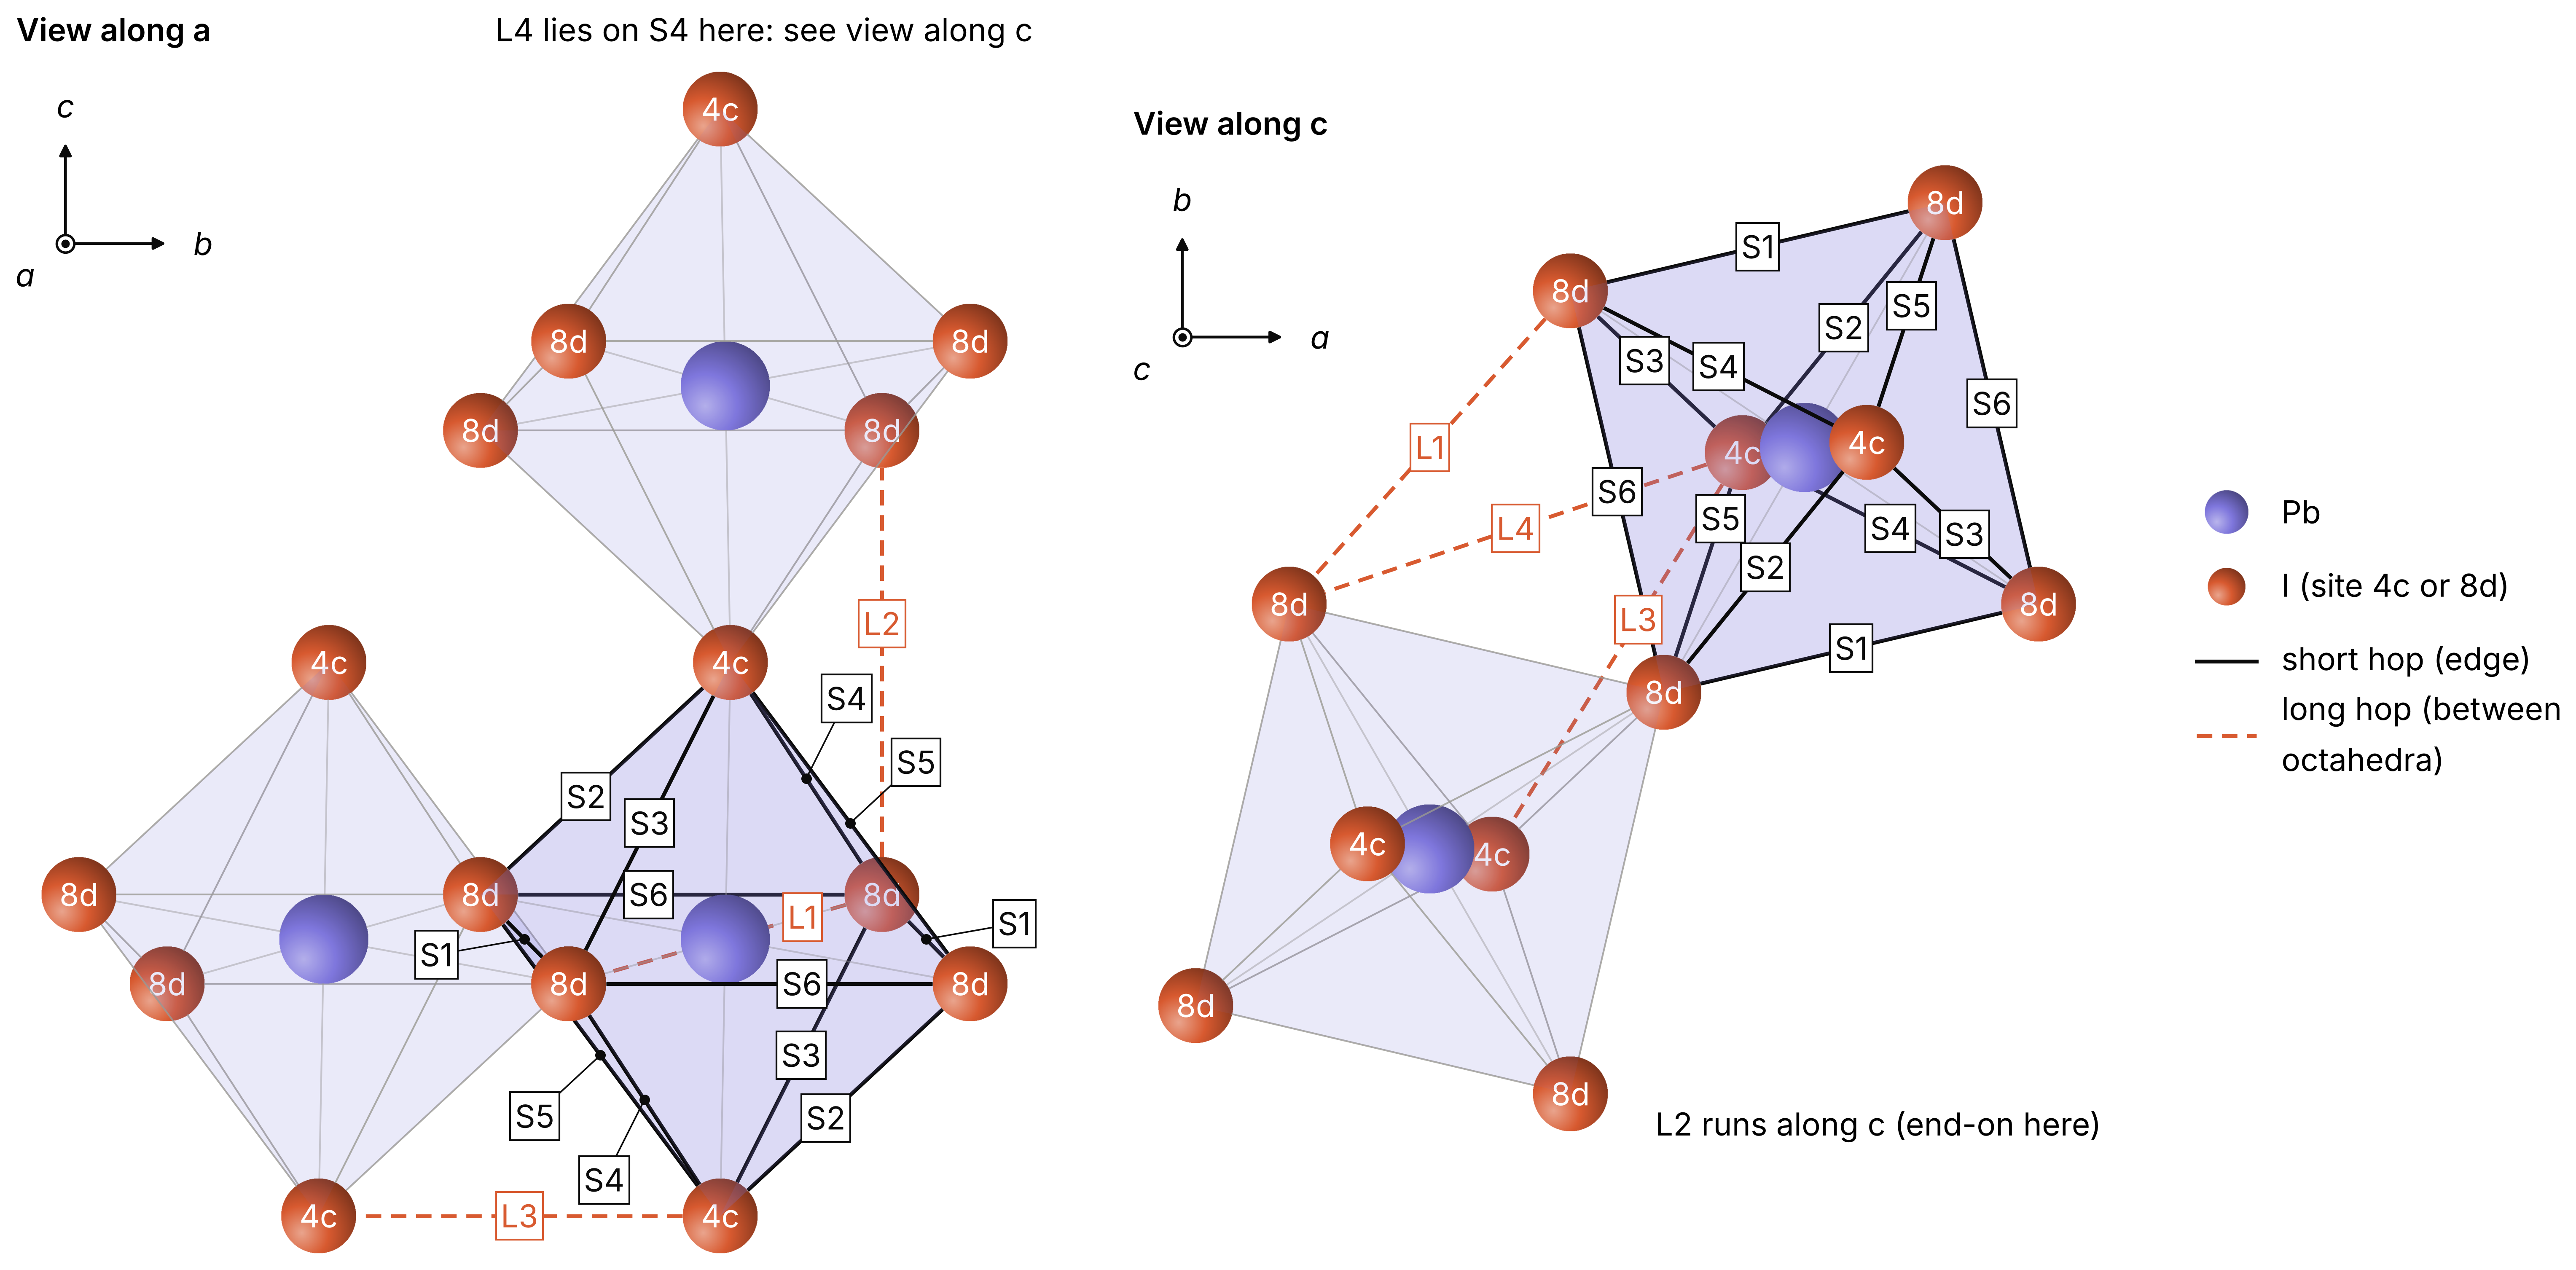
\includegraphics[width=\textwidth,height=0.83\textheight,keepaspectratio]{octahedra_hops_wide.png}
  \refs{S1--S6: along octahedron edges; L1--L4: between corner-sharing octahedra. Figure, hop set and lengths: this work (tight-relaxed cell).}
\end{frame}

\begin{frame}{The ten hops: how many, and where they go}
  \centering\footnotesize
  \begin{tabular}{llcccl}
    \toprule
    Hop & Ends & Length (\AA) & From 8d & From 4c & Moves the vacancy \\
    \midrule
    S1, S6 & 8d--8d & 4.41, 4.60 & 2 each & 0 & within a PbI$_2$ layer \\
    S2--S5 & 4c--8d & 4.43--4.56 & 1 each & 2 each & PbI$_2$ $\leftrightarrow$ CsI layer \\
    L1 & 8d--8d & 4.80 & 1 & 0 & within a PbI$_2$ layer \\
    L2 & 8d--8d & 5.18 & 1 & 0 & straight along $c$ \\
    L3 & 4c--4c & 5.28 & 0 & 2 & within a CsI layer \\
    L4 & 4c--8d & 5.93 & 1 & 2 & between layers \\
    \midrule
    Total & & & 11 & 12 & \\
    \bottomrule
  \end{tabular}

  \vspace{0.3em}
  \raggedright\footnotesize
  \begin{itemize}
    \item Half of the short hops from 8d lead to 4c; a 4c vacancy has \textbf{no short hop to another 4c}
    \item ab plane: 8d--8d hops are enough. Along $c$: needs \textbf{4c--8d hops} (8d$\rightarrow$4c$\rightarrow$8d) or the long L2
    \item $\Rightarrow$ transport depends on barriers \emph{and} hop numbers \emph{and} 4c/8d site energies: anisotropic diffusion
  \end{itemize}
  \refs{Hop set, counts and directions: this work (\texttt{hop\_network.py}, perfect supercell). Paper A treats one barrier per type\cit{1}.\quad \RA}
\end{frame}

\begin{frame}{NEB scope: start with hops that have published values}
  \footnotesize
  \begin{tabular}{llll}
    \toprule
    Published path & Value & Our hop & How identified \\
    \midrule
    Paper A: 4c--4c\cit{1} & 0.77 eV & \textbf{L3} & only 4c--4c hop \\
    Paper A: 8d--8d edge\cit{1} & 0.34 eV & S1 or S6 & schematic figure only \\
    Paper A: 8d--4c edge\cit{1} & 0.35 eV & one of S2--S5 & schematic figure only \\
    Zhang: in-plane\cit{20} & 0.54 eV & \textbf{S1} (probable) & rises $\approx$1 \AA\ along $c$ (S6: 0) \\
    Zhang: out-of-plane\cit{20} & 0.51 eV & \textbf{S2} (probable) & rises $\approx$2.7 \AA, no sideways shift \\
    \bottomrule
  \end{tabular}

  \vspace{0.1em}
  \begin{tabular}{clp{0.52\textwidth}}
    \toprule
    Stage & Hops & Purpose \\
    \midrule
    1 & S1, S2, L3, S6 & Compare with published values; S1 vs S6 = first spread within a type \\
    2 & S3, S4, S5 & Spread of the 4c--8d hops (control transport along $c$) \\
    3 & L1, L2, L4 & Only if the network analysis needs them \\
    \bottomrule
  \end{tabular}

  \vspace{0.1em}
  Spread $<$ 0.03 eV $\Rightarrow$ one barrier per type. Small threshold: at 300 K, 0.05 eV changes a rate $\approx 7\times$.
  \refs{\RA\quad \RT\ (paths assigned from its Fig.~6a,b; raster figure, $\pm$0.3 \AA).}
\end{frame}

% =====================================================================
\section{Next steps}

\begin{frame}{NEB: ready to run}
  \small
  \textbf{\texttt{build\_neb.py}} (written and tested)
  \begin{itemize}
    \item End points \alert{by symmetry}: the relaxed 4c and 8d vacancies are mapped onto any site with the 64 Pnma operations\cit{17} $\rightarrow$ no extra relaxations
    \item Atoms renumbered so only the hopping iodine moves; IDPP starting path\cit{16,18}
  \end{itemize}

  \textbf{NEB settings and why}
  \begin{tabular}{lll}
    \toprule
    Climbing image & on & Gives the true saddle point\cit{15} \\
    Intermediate images & 4 & Spacing about 1 \AA; the climbing image finds the saddle \\
    $k$-mesh & 2$\times$2$\times$2 & Same as the end points (2$\times$2$\times$1 rejected) \\
    Barrier reported & both directions & Plus the average, to compare with paper A\cit{1} \\
    \bottomrule
  \end{tabular}

  \vspace{0.6em}
  \textbf{First run:} S1 (8d--8d, $+1$), against paper A's 0.34 eV.
  \refs{\RA\quad \RO\quad \RP\quad \RQ\quad \RR}
\end{frame}

\begin{frame}{Plan}
  \begin{enumerate}
    \item Finish the neutral 4c relaxation $\rightarrow$ final neutral site energy
    \item NEB stage 1 ($+1$): S1, S2, L3, S6 (published comparisons); stage 2: S3, S4, S5
    \item Long hops L1, L2, L4 only if the network analysis needs them
    \item Neutral NEB for the stage-1 hops
    \item Build the CsI-terminated (001) slab: symmetric, all atoms free; 11 layers, 15-layer test
    \item Vacancy energies and barriers layer by layer, until they return to the bulk values
  \end{enumerate}
\end{frame}

\begin{frame}{Questions for discussion}
  \begin{enumerate}
    \item \textbf{Paper A's lattice\cit{1}:} rerun our $+1$ pair on their cell (8.68/8.71/12.44 \AA) to test the tilt explanation? Cost: two relaxations, about one week.
    \item \textbf{Neutral vacancy:} is a hybrid-functional check of the delocalised electron worth the cost?
    \item \textbf{Spin--orbit coupling:} single-point check on the site energies now, or after the barriers?
    \item \textbf{NEB scope:} start with the 4 hops comparable to published values, then decide; neutral only for stage 1?
    \item Contact paper A's authors about their charge state and 4c/8d end-point energies?
  \end{enumerate}
  \refs{\RA}
\end{frame}

\begin{frame}{Summary}
  \begin{itemize}
    \item \textbf{Bulk reference built:} converged settings, tight lattice, perfect and vacancy supercells.
    \item \textbf{Site preference depends on charge:} $+1$ degenerate ($-1$ meV); neutral favours 4c by $\geq 36$ meV, opposite to paper A.
    \item \textbf{Neutral vacancy is a shallow donor} in PBEsol (moment $0\,\mu_B$).
    \item \textbf{Benchmark mismatch} likely from paper A's nearly square, less-tilted cell.
    \item \textbf{Ten distinct hops}; transport along $c$ needs 4c--8d hops $\Rightarrow$ staged NEB plan, inputs ready.
  \end{itemize}

  \vspace{1em}
  \centering
  \textbf{Next: first barrier (S1) against paper A's 0.34 eV.}
\end{frame}

\begin{frame}[allowframebreaks]{References}
  \tiny
  \begin{itemize}\setlength{\itemsep}{1pt}
    \item[] \RA
    \item[] \RB
    \item[] \RC
    \item[] \RD
    \item[] \RE
    \item[] \RF
    \item[] \RG
    \item[] \RH
    \item[] \RI
    \item[] \RJ
    \item[] \RK
    \item[] \RL
    \item[] \RM
    \item[] \RN
    \item[] \RO
    \item[] \RP
    \item[] \RQ
    \item[] \RR
    \item[] \RS
    \item[] \RT
  \end{itemize}
\end{frame}

\end{document}
